\chapter{Конструкторская часть}

В данном разделе выполняется проектирование базы данных и архитектуры программного обеспечения для хранения и обработки стоматологических снимков челюсти человека. Описываются сущности базы данных, связи между ними, ограничения целостности, ролевая модель, схемы алгоритмов проектируемых триггеров и функций, а также архитектурные диаграммы системы.

\section{Архитектура системы}

Для описания архитектуры программного комплекса используется модель C4. Она позволяет рассматривать систему на нескольких уровнях детализации: от общего контекста до отдельных компонентов и классов.

\subsection{Уровень L1: контекст системы}

На уровне контекста разрабатываемая система рассматривается как единый программный комплекс, с которым взаимодействуют пользователи: врач-стоматолог, рентгенолог и администратор. Система использует PostgreSQL для долговременного хранения данных и Redis для внешнего кэширования часто запрашиваемой информации.

Контекстная диаграмма системы приведена на рисунке~\ref{fig:c4-context}.

\begin{figure}[H]
	\centering
	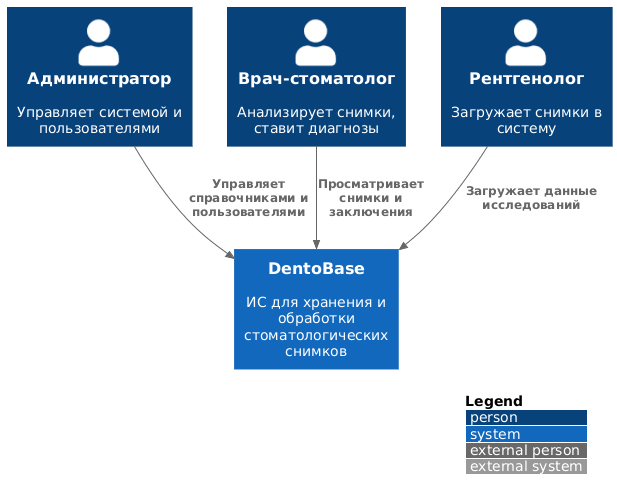
\includegraphics[width=0.7\textwidth]{context}
	\caption{C4 L1 --- контекст системы}
	\label{fig:c4-context}
\end{figure}

\subsection{Уровень L2: контейнеры}

На уровне контейнеров система разделяется на технологический пользовательский интерфейс, компонент бизнес-логики, базу данных PostgreSQL и InMemory-хранилище Redis. Технологический пользовательский интерфейс используется для системного тестирования вариантов использования и работает с тем же компонентом бизнес-логики, с которым в дальнейшем будет работать полноценный графический интерфейс.

Диаграмма контейнеров приведена на рисунке~\ref{fig:c4-containers}.

\begin{figure}[H]
	\centering
	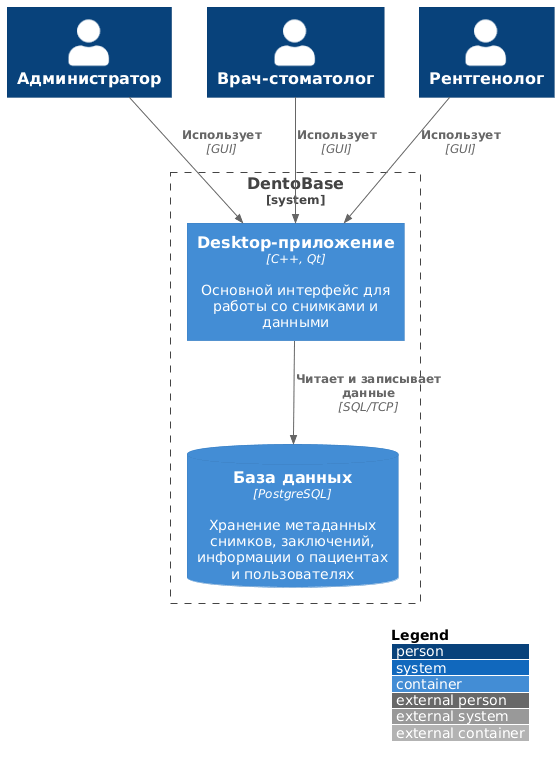
\includegraphics[width=0.7\textwidth]{containers}
	\caption{C4 L2 --- диаграмма контейнеров}
	\label{fig:c4-containers}
\end{figure}

\subsection{Уровень L3: компоненты}

На уровне компонентов выделяются пользовательский интерфейс, сервисы бизнес-логики, интерфейсы репозиториев, PostgreSQL-реализации репозиториев, SQL-builder-ы и компонент кэширования. Такое разделение позволяет отделить бизнес-логику от деталей хранения данных и упростить замену пользовательского интерфейса.

Диаграмма компонентов приведена на рисунке~\ref{fig:c4-components}.

\begin{figure}[H]
	\centering
	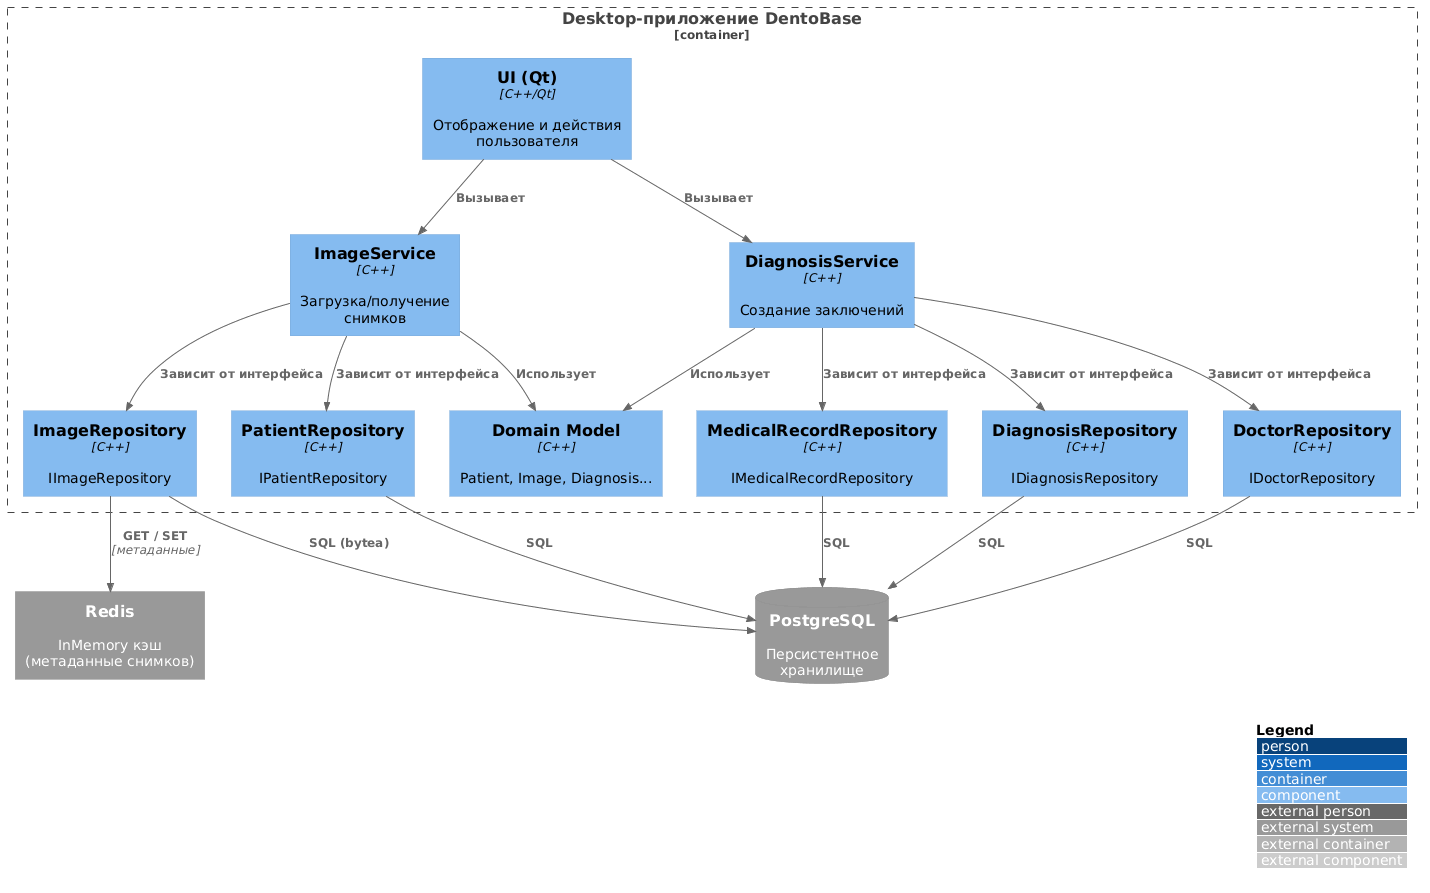
\includegraphics[width=\textwidth]{comp}
	\caption{C4 L3 --- диаграмма компонентов}
	\label{fig:c4-components}
\end{figure}

\subsection{Уровень L4: компоненты технологического интерфейса}

Технологический пользовательский интерфейс реализуется в виде консольного приложения. Он предназначен для проверки всех основных вариантов использования системы без разработки полноценного графического интерфейса. При этом технологический интерфейс не обращается к базе данных напрямую, а использует интерфейс прикладного сервиса. Это позволяет соблюдать принцип инверсии зависимостей и переиспользовать бизнес-логику в будущем графическом интерфейсе.

Диаграмма компонентов технологического интерфейса приведена на рисунке~\ref{fig:tech-ui-l4}.

\begin{figure}[H]
	\centering
	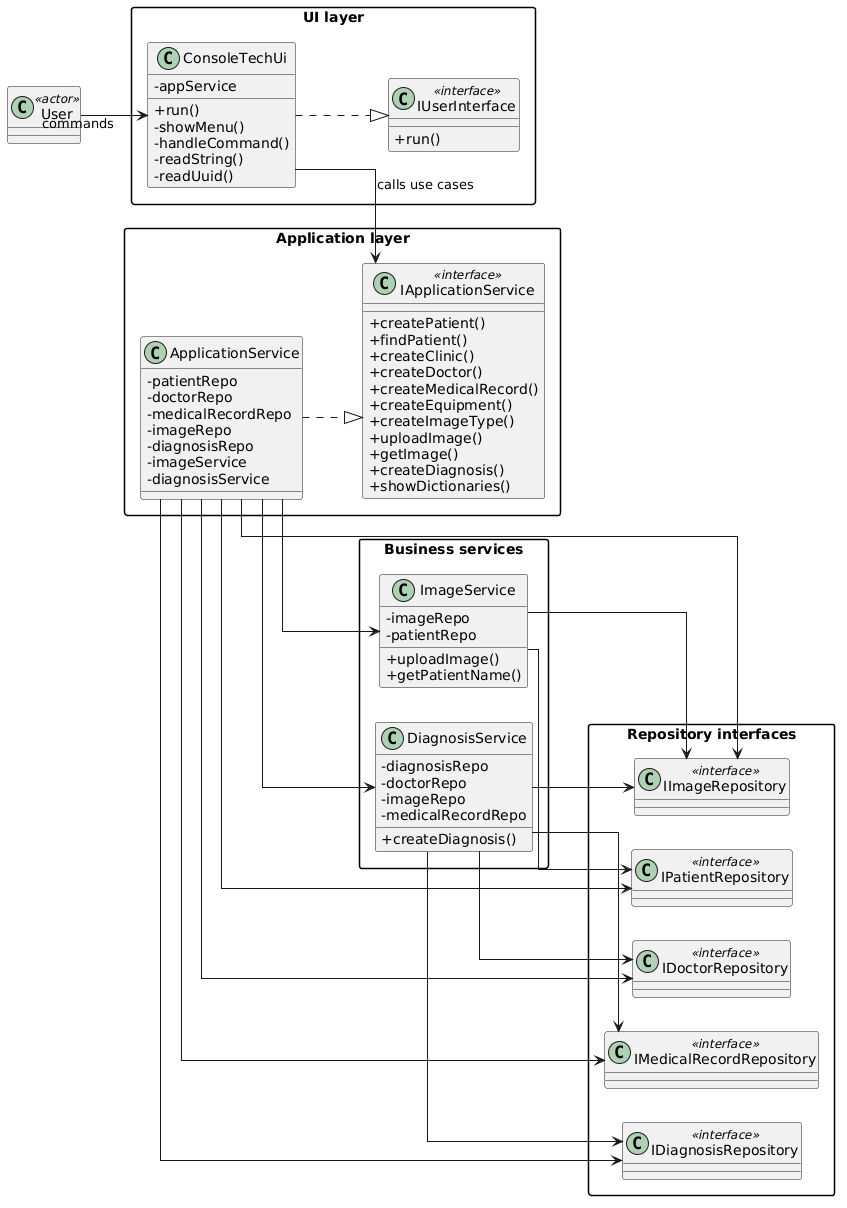
\includegraphics[width=0.75\textwidth]{tech_ui_l4}
	\caption{C4 L4 --- компоненты технологического пользовательского интерфейса}
	\label{fig:tech-ui-l4}
\end{figure}

\section{Диаграмма классов приложения}

Приложение строится с разделением на доменный слой, слой репозиториев, слой бизнес-сервисов и слой пользовательского интерфейса. Доменный слой содержит структуры предметной области. Репозитории отвечают за доступ к данным. Сервисы реализуют бизнес-операции, а пользовательский интерфейс инициирует сценарии работы пользователя.

Полная диаграмма классов приложения приведена на рисунке~\ref{fig:classes-design}.

\begin{figure}[H]
	\centering
	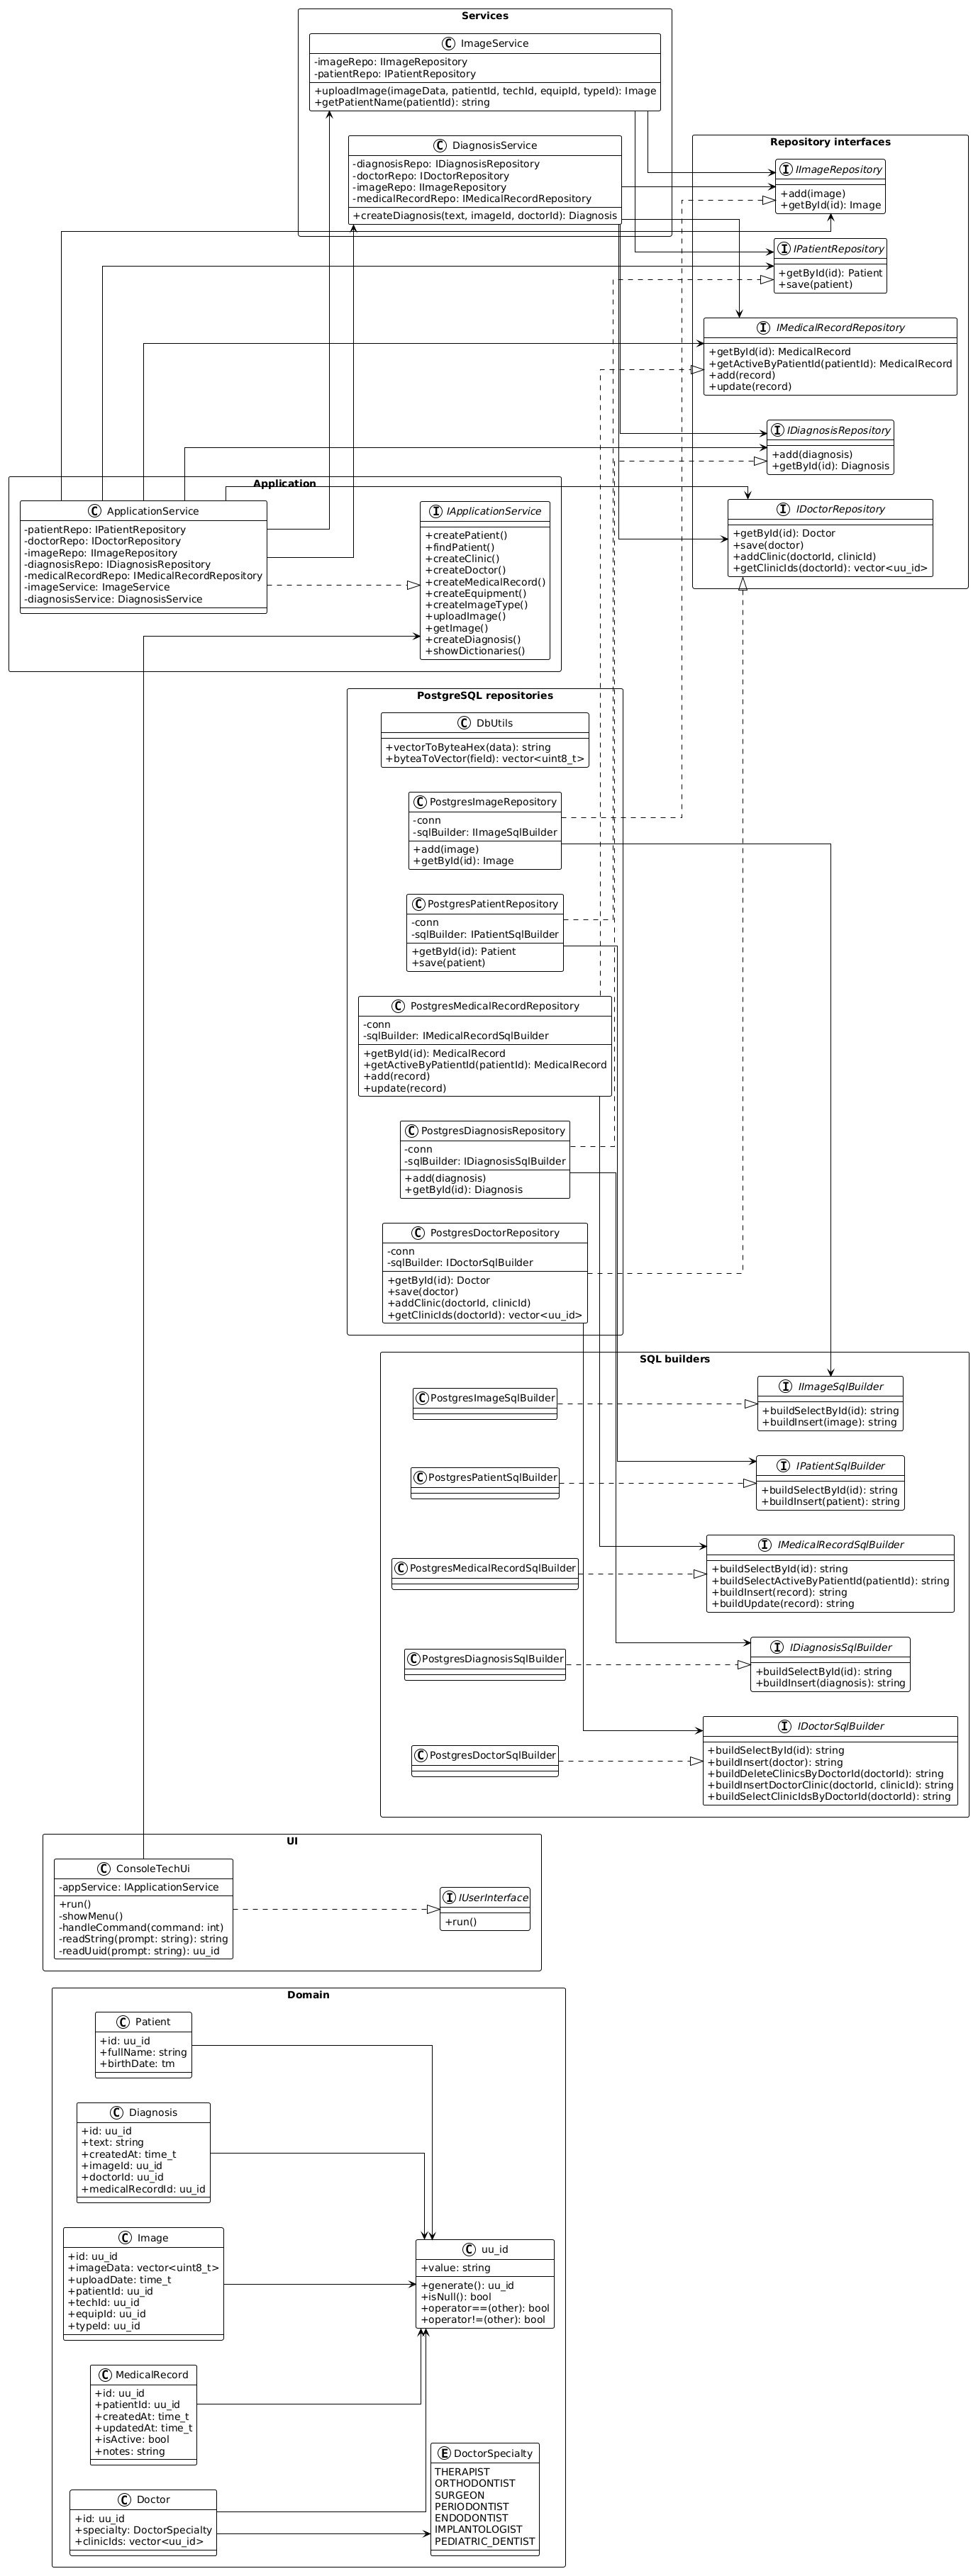
\includegraphics[width=0.5\textwidth]{classes}
	\caption{Диаграмма классов приложения}
	\label{fig:classes-design}
\end{figure}

В архитектуре приложения используются следующие принципы:
\begin{itemize}
	\item зависимость бизнес-логики от абстракций репозиториев, а не от конкретной реализации PostgreSQL;
	\item разделение доменных моделей, сервисов и слоя доступа к данным;
	\item возможность замены технологического интерфейса на графический интерфейс без изменения бизнес-логики;
	\item инкапсуляция SQL-запросов в отдельных SQL-builder-ах.
\end{itemize}

\section{Проектирование базы данных}

Проектируемая база данных предназначена для хранения сведений о пациентах, врачах, клиниках, лаборантах, оборудовании, типах снимков, медицинских картах, стоматологических снимках и врачебных заключениях.

Диаграмма проектируемой базы данных приведена на рисунке~\ref{fig:db-schema-design}.

\begin{figure}[H]
	\centering
	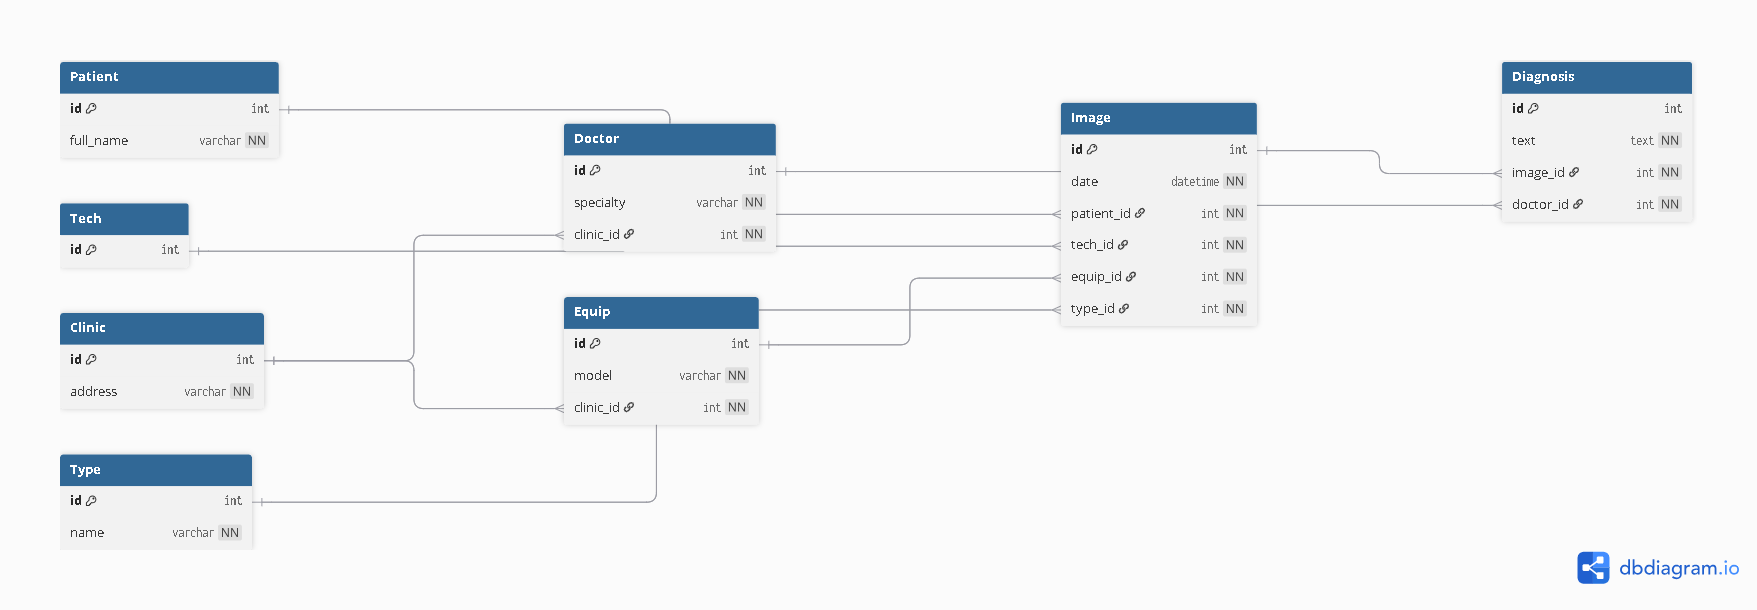
\includegraphics[width=\textwidth]{DB}
	\caption{Диаграмма проектируемой базы данных}
	\label{fig:db-schema-design}
\end{figure}

В базе данных выделены следующие таблицы:
\begin{itemize}
	\item \texttt{patients} --- пациенты;
	\item \texttt{clinics} --- стоматологические клиники;
	\item \texttt{doctors} --- врачи;
	\item \texttt{doctor\_clinics} --- ассоциативная таблица связи врачей и клиник;
	\item \texttt{technicians} --- лаборанты;
	\item \texttt{equipment} --- оборудование;
	\item \texttt{image\_types} --- типы снимков;
	\item \texttt{images} --- стоматологические снимки;
	\item \texttt{medical\_records} --- медицинские карты;
	\item \texttt{diagnoses} --- врачебные заключения.
\end{itemize}

Связь между врачами и клиниками является связью многие-ко-многим. Один врач может работать в нескольких клиниках, а в одной клинике может работать несколько врачей. Для реализации данной связи введена таблица \texttt{doctor\_clinics}, содержащая внешние ключи на таблицы \texttt{doctors} и \texttt{clinics}.

\section{Описание сущностей базы данных}

В таблице~\ref{tab:patients-design} приведено описание таблицы \texttt{patients}.

\begin{table}[H]
	\caption{Описание таблицы patients}
	\label{tab:patients-design}
	\centering
	\begin{tabular}{|p{0.24\textwidth}|p{0.22\textwidth}|p{0.24\textwidth}|p{0.20\textwidth}|}
		\hline
		Столбец & Тип данных & Ограничения & Значение \\
		\hline
		id & UUID & PRIMARY KEY, NOT NULL & идентификатор пациента \\
		\hline
		full\_name & TEXT & NOT NULL & ФИО пациента \\
		\hline
		birth\_date & DATE & NOT NULL & дата рождения \\
		\hline
	\end{tabular}
\end{table}

В таблице~\ref{tab:clinics-design} приведено описание таблицы \texttt{clinics}.

\begin{table}[H]
	\caption{Описание таблицы clinics}
	\label{tab:clinics-design}
	\centering
	\begin{tabular}{|p{0.24\textwidth}|p{0.22\textwidth}|p{0.24\textwidth}|p{0.20\textwidth}|}
		\hline
		Столбец & Тип данных & Ограничения & Значение \\
		\hline
		id & UUID & PRIMARY KEY, NOT NULL & идентификатор клиники \\
		\hline
		address & TEXT & NOT NULL & адрес клиники \\
		\hline
	\end{tabular}
\end{table}

В таблице~\ref{tab:doctors-design} приведено описание таблицы \texttt{doctors}.

\begin{table}[H]
	\caption{Описание таблицы doctors}
	\label{tab:doctors-design}
	\centering
	\begin{tabular}{|p{0.24\textwidth}|p{0.22\textwidth}|p{0.24\textwidth}|p{0.20\textwidth}|}
		\hline
		Столбец & Тип данных & Ограничения & Значение \\
		\hline
		id & UUID & PRIMARY KEY, NOT NULL & идентификатор врача \\
		\hline
		specialty & TEXT & NOT NULL & специальность врача \\
		\hline
	\end{tabular}
\end{table}

В таблице~\ref{tab:doctor-clinics-design} приведено описание таблицы \texttt{doctor\_clinics}.

\begin{table}[H]
	\caption{Описание таблицы doctor\_clinics}
	\label{tab:doctor-clinics-design}
	\centering
	\begin{tabular}{|p{0.24\textwidth}|p{0.22\textwidth}|p{0.24\textwidth}|p{0.20\textwidth}|}
		\hline
		Столбец & Тип данных & Ограничения & Значение \\
		\hline
		doctor\_id & UUID & PRIMARY KEY, FOREIGN KEY, NOT NULL & идентификатор врача \\
		\hline
		clinic\_id & UUID & PRIMARY KEY, FOREIGN KEY, NOT NULL & идентификатор клиники \\
		\hline
	\end{tabular}
\end{table}

В таблице~\ref{tab:technicians-design} приведено описание таблицы \texttt{technicians}.

\begin{table}[H]
	\caption{Описание таблицы technicians}
	\label{tab:technicians-design}
	\centering
	\begin{tabular}{|p{0.24\textwidth}|p{0.22\textwidth}|p{0.24\textwidth}|p{0.20\textwidth}|}
		\hline
		Столбец & Тип данных & Ограничения & Значение \\
		\hline
		id & UUID & PRIMARY KEY, NOT NULL & идентификатор лаборанта \\
		\hline
		full\_name & TEXT & NOT NULL & ФИО лаборанта \\
		\hline
		clinic\_id & UUID & FOREIGN KEY & клиника работы \\
		\hline
	\end{tabular}
\end{table}

В таблице~\ref{tab:equipment-design} приведено описание таблицы \texttt{equipment}.

\begin{table}[H]
	\caption{Описание таблицы equipment}
	\label{tab:equipment-design}
	\centering
	\begin{tabular}{|p{0.24\textwidth}|p{0.22\textwidth}|p{0.24\textwidth}|p{0.20\textwidth}|}
		\hline
		Столбец & Тип данных & Ограничения & Значение \\
		\hline
		id & UUID & PRIMARY KEY, NOT NULL & идентификатор оборудования \\
		\hline
		model & TEXT & NOT NULL & модель оборудования \\
		\hline
		clinic\_id & UUID & FOREIGN KEY & клиника размещения \\
		\hline
	\end{tabular}
\end{table}

В таблице~\ref{tab:image-types-design} приведено описание таблицы \texttt{image\_types}.

\begin{table}[H]
	\caption{Описание таблицы image\_types}
	\label{tab:image-types-design}
	\centering
	\begin{tabular}{|p{0.24\textwidth}|p{0.22\textwidth}|p{0.24\textwidth}|p{0.20\textwidth}|}
		\hline
		Столбец & Тип данных & Ограничения & Значение \\
		\hline
		id & UUID & PRIMARY KEY, NOT NULL & идентификатор типа снимка \\
		\hline
		name & TEXT & UNIQUE, NOT NULL & название типа снимка \\
		\hline
	\end{tabular}
\end{table}

В таблице~\ref{tab:images-design} приведено описание таблицы \texttt{images}. Для хранения бинарных данных снимка используется тип \texttt{BYTEA}, предназначенный для хранения двоичных строк в PostgreSQL~\cite{postgresql-bytea}.

\begin{table}[H]
	\caption{Описание таблицы images}
	\label{tab:images-design}
	\centering
	\small
	\begin{tabular}{|p{0.23\textwidth}|p{0.20\textwidth}|p{0.25\textwidth}|p{0.22\textwidth}|}
		\hline
		Столбец & Тип данных & Ограничения & Значение \\
		\hline
		id & UUID & PRIMARY KEY, NOT NULL & идентификатор снимка \\
		\hline
		image\_data & BYTEA & NOT NULL & бинарные данные снимка \\
		\hline
		upload\_date & TIMESTAMP & NOT NULL & дата загрузки \\
		\hline
		patient\_id & UUID & FOREIGN KEY & пациент \\
		\hline
		tech\_id & UUID & FOREIGN KEY & лаборант \\
		\hline
		equip\_id & UUID & FOREIGN KEY & оборудование \\
		\hline
		type\_id & UUID & FOREIGN KEY & тип снимка \\
		\hline
	\end{tabular}
\end{table}

В таблице~\ref{tab:medical-records-design} приведено описание таблицы \texttt{medical\_records}.

\begin{table}[H]
	\caption{Описание таблицы medical\_records}
	\label{tab:medical-records-design}
	\centering
	\small
	\begin{tabular}{|p{0.23\textwidth}|p{0.20\textwidth}|p{0.25\textwidth}|p{0.22\textwidth}|}
		\hline
		Столбец & Тип данных & Ограничения & Значение \\
		\hline
		id & UUID & PRIMARY KEY, NOT NULL & идентификатор медицинской карты \\
		\hline
		patient\_id & UUID & FOREIGN KEY & пациент \\
		\hline
		created\_at & TIMESTAMP & NOT NULL & дата создания \\
		\hline
		updated\_at & TIMESTAMP & NOT NULL & дата обновления \\
		\hline
		is\_active & BOOLEAN & NOT NULL & признак активности \\
		\hline
		notes & TEXT & --- & примечания \\
		\hline
	\end{tabular}
\end{table}

В таблице~\ref{tab:diagnoses-design} приведено описание таблицы \texttt{diagnoses}.

\begin{table}[H]
	\caption{Описание таблицы diagnoses}
	\label{tab:diagnoses-design}
	\centering
	\small
	\begin{tabular}{|p{0.23\textwidth}|p{0.20\textwidth}|p{0.25\textwidth}|p{0.22\textwidth}|}
		\hline
		Столбец & Тип данных & Ограничения & Значение \\
		\hline
		id & UUID & PRIMARY KEY, NOT NULL & идентификатор диагноза \\
		\hline
		text & TEXT & NOT NULL & текст заключения \\
		\hline
		created\_at & TIMESTAMP & NOT NULL & дата создания \\
		\hline
		image\_id & UUID & UNIQUE, FOREIGN KEY & снимок \\
		\hline
		doctor\_id & UUID & FOREIGN KEY & врач \\
		\hline
		medical\_record\_id & UUID & FOREIGN KEY & медицинская карта \\
		\hline
	\end{tabular}
\end{table}

\section{Ограничения целостности}

Ограничения целостности используются для предотвращения появления некорректных данных в базе данных. PostgreSQL поддерживает первичные ключи, внешние ключи, уникальные ограничения, ограничения \texttt{NOT NULL} и проверочные ограничения~\cite{postgresql-constraints}.

В проектируемой базе данных используются следующие ограничения:
\begin{itemize}
	\item первичные ключи для однозначной идентификации записей;
	\item внешние ключи для обеспечения ссылочной целостности;
	\item ограничения \texttt{NOT NULL} для обязательных атрибутов;
	\item уникальное ограничение для названий типов снимков;
	\item уникальное ограничение для связи снимка и диагноза;
	\item составной первичный ключ в таблице \texttt{doctor\_clinics};
	\item каскадное удаление записей ассоциативной таблицы при удалении врача или клиники.
\end{itemize}

Ограничения ссылочной целостности позволяют гарантировать, что снимок не будет ссылаться на несуществующего пациента, оборудование или тип снимка, а диагноз не будет ссылаться на несуществующего врача, снимок или медицинскую карту.

\section{Проверка соответствия базы данных третьей нормальной форме}

Отношение находится в первой нормальной форме, если все значения его атрибутов атомарны. Все таблицы проектируемой базы данных содержат атомарные значения: идентификаторы, текстовые строки, даты, логические значения и бинарные данные снимка.

Отношение находится во второй нормальной форме, если оно находится в первой нормальной форме и каждый неключевой атрибут функционально полно зависит от всего первичного ключа. В большинстве таблиц первичный ключ состоит из одного атрибута \texttt{id}, поэтому частичная зависимость невозможна. Таблица \texttt{doctor\_clinics} имеет составной первичный ключ, но не содержит неключевых атрибутов.

Отношение находится в третьей нормальной форме, если оно находится во второй нормальной форме и не содержит транзитивных зависимостей неключевых атрибутов от первичного ключа~\cite{date-db}. В проектируемой базе данных данные разных сущностей вынесены в отдельные таблицы. Например, адрес клиники хранится только в таблице \texttt{clinics}, а в таблицах \texttt{equipment}, \texttt{technicians} и \texttt{doctor\_clinics} используются только ссылки на клинику.

Проверка соответствия таблиц третьей нормальной форме приведена в таблице~\ref{tab:3nf}.

\begin{table}[H]
	\caption{Проверка соответствия таблиц 3НФ}
	\label{tab:3nf}
	\centering
	\small
	\begin{tabular}{|p{0.26\textwidth}|p{0.64\textwidth}|}
		\hline
		Таблица & Обоснование \\
		\hline
		patients & все неключевые атрибуты зависят только от идентификатора пациента \\
		\hline
		clinics & адрес зависит только от идентификатора клиники \\
		\hline
		doctors & специальность зависит только от идентификатора врача \\
		\hline
		doctor\_clinics & таблица не содержит неключевых атрибутов \\
		\hline
		technicians & ФИО и клиника зависят только от идентификатора лаборанта \\
		\hline
		equipment & модель и клиника размещения зависят только от идентификатора оборудования \\
		\hline
		image\_types & название типа снимка зависит только от идентификатора типа \\
		\hline
		images & данные снимка и метаданные зависят только от идентификатора снимка \\
		\hline
		medical\_records & атрибуты медицинской карты зависят только от идентификатора карты \\
		\hline
		diagnoses & текст заключения и связи зависят только от идентификатора диагноза \\
		\hline
	\end{tabular}
\end{table}

Таким образом, проектируемая база данных находится в третьей нормальной форме.

\section{Ролевая модель базы данных}

Ролевая модель на уровне базы данных предназначена для разграничения доступа пользователей к данным. PostgreSQL поддерживает создание ролей и выдачу прав доступа к объектам базы данных~\cite{postgresql-privileges}.

В системе проектируются следующие роли:
\begin{itemize}
	\item \texttt{dentobase\_admin} --- администратор;
	\item \texttt{dentobase\_doctor} --- врач-стоматолог;
	\item \texttt{dentobase\_technician} --- рентгенолог или лаборант.
\end{itemize}

Описание прав доступа приведено в таблице~\ref{tab:db-roles}.

\begin{table}[H]
	\caption{Ролевая модель базы данных}
	\label{tab:db-roles}
	\centering
	\small
	\begin{tabular}{|p{0.25\textwidth}|p{0.65\textwidth}|}
		\hline
		Роль & Права доступа \\
		\hline
		dentobase\_admin & полный доступ ко всем таблицам и справочникам \\
		\hline
		dentobase\_doctor & просмотр пациентов, медицинских карт и снимков; добавление диагнозов; просмотр справочников \\
		\hline
		dentobase\_technician & добавление пациентов и снимков; просмотр типов снимков, оборудования и клиник \\
		\hline
	\end{tabular}
\end{table}

Такая ролевая модель соответствует выделенным в аналитической части группам пользователей и позволяет ограничивать доступ к медицинским данным на уровне СУБД.

\section{Проектирование триггеров и функций базы данных}

Для автоматизации обработки данных на стороне базы данных проектируются триггер обновления даты изменения медицинской карты и функция получения списка снимков пациента. Триггеры PostgreSQL позволяют автоматически выполнять заданную функцию при наступлении события вставки, изменения или удаления записи~\cite{postgresql-triggers}.

\subsection{Триггер обновления даты изменения медицинской карты}

При изменении медицинской карты необходимо автоматически обновлять поле \texttt{updated\_at}. Это позволяет фиксировать момент последнего изменения карты независимо от клиентского приложения.

Схема алгоритма триггера приведена на рисунке~\ref{fig:trigger-medical-record}.

\begin{figure}[H]
	\centering
	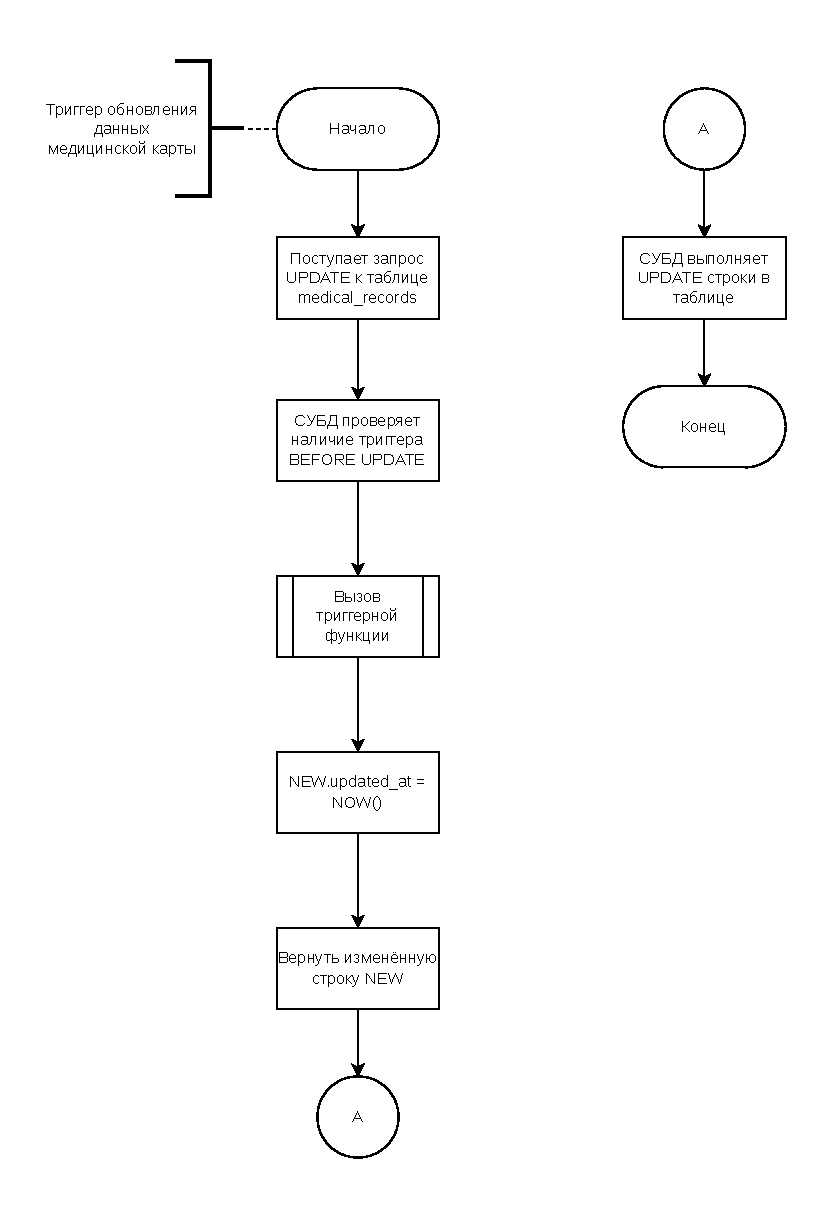
\includegraphics[width=0.7\textwidth]{trigger_medrec}
	\caption{Схема алгоритма триггера обновления даты медицинской карты}
	\label{fig:trigger-medical-record}
\end{figure}

Алгоритм работы триггера:
\begin{enumerate}
	\item пользователь или приложение инициирует обновление медицинской карты;
	\item СУБД вызывает триггер перед изменением строки;
	\item в поле \texttt{updated\_at} записывается текущее время;
	\item обновленная строка сохраняется в таблице \texttt{medical\_records}.
\end{enumerate}

\subsection{Функция получения снимков пациента}

Для просмотра истории снимков пациента проектируется функция получения снимков пациента. Она принимает идентификатор пациента и возвращает список его снимков с датой загрузки, типом снимка и моделью оборудования.

Схема алгоритма функции приведена на рисунке~\ref{fig:function-patient-images}.

\begin{figure}[H]
	\centering
	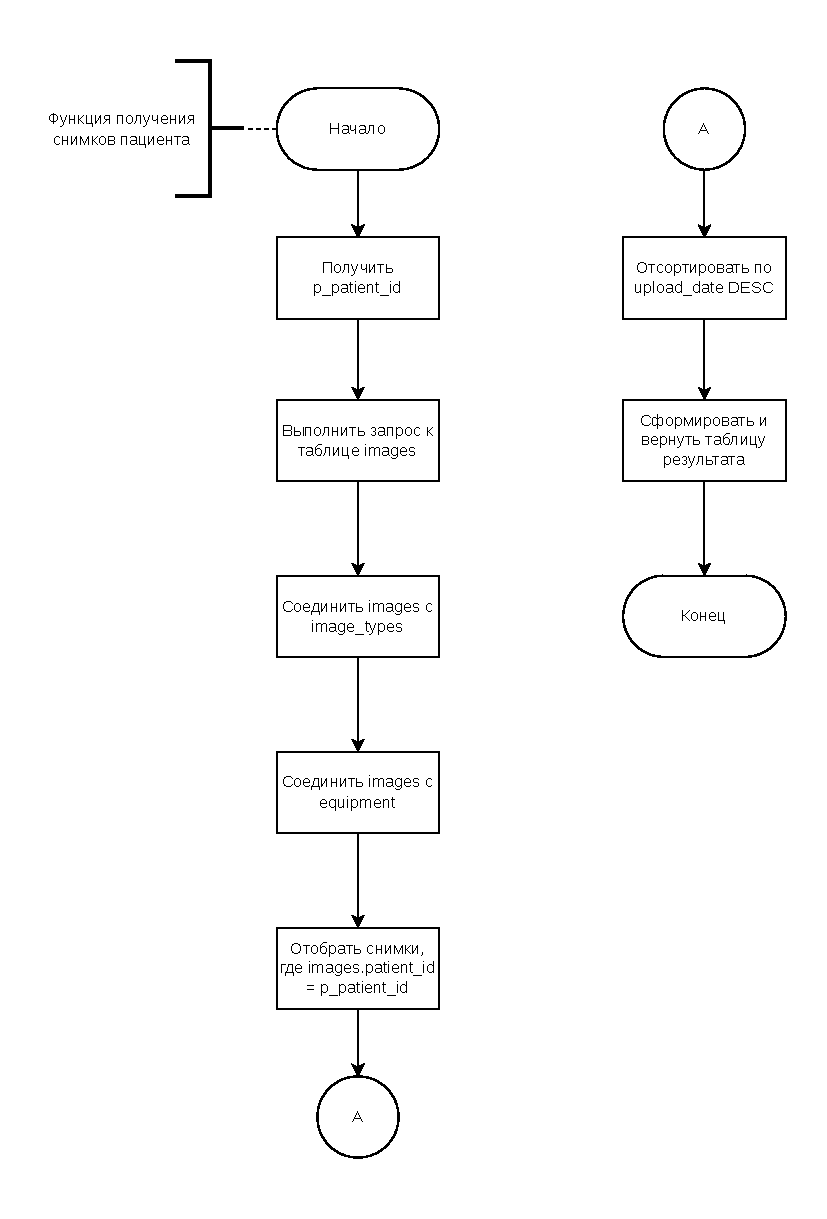
\includegraphics[width=0.75\textwidth]{func}
	\caption{Схема алгоритма функции получения снимков пациента}
	\label{fig:function-patient-images}
\end{figure}

Алгоритм работы функции:
\begin{enumerate}
	\item функция получает идентификатор пациента;
	\item выполняется поиск снимков, связанных с данным пациентом;
	\item для каждого снимка подставляются сведения о типе снимка и оборудовании;
	\item результат сортируется по дате загрузки;
	\item функция возвращает табличный результат.
\end{enumerate}

\section{Проектирование внешнего кэширования}

Для ускорения доступа к часто запрашиваемым данным проектируется использование внешнего InMemory-хранилища Redis. Redis применяется как кэш между бизнес-логикой приложения и PostgreSQL~\cite{redis-docs}.

Кэширование целесообразно использовать для следующих данных:
\begin{itemize}
	\item имя пациента по идентификатору;
	\item метаданные снимка;
	\item список снимков пациента;
	\item справочники типов снимков.
\end{itemize}

Общая схема работы кэша:
\begin{enumerate}
	\item приложение формирует ключ кэша;
	\item выполняется поиск значения в Redis;
	\item если значение найдено, оно возвращается без обращения к PostgreSQL;
	\item если значение отсутствует, данные читаются из PostgreSQL;
	\item результат сохраняется в Redis и возвращается приложению.
\end{enumerate}

\clearpage

Диаграмма взаимодействия PostgreSQL и Redis приведена на рисунке~\ref{fig:redis-sequence}.

\begin{figure}[H]
	\centering
	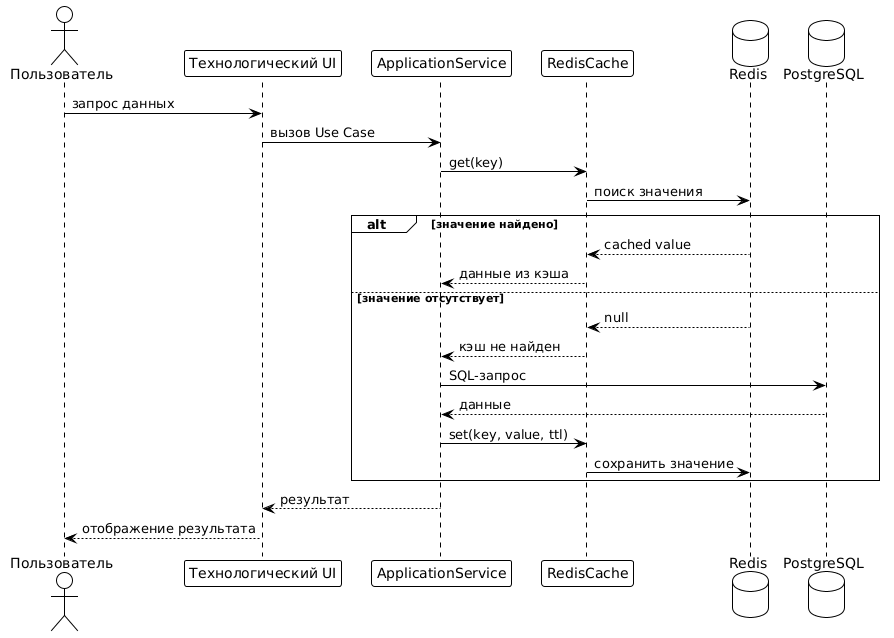
\includegraphics[width=\textwidth]{redis_sequence}
	\caption{Схема взаимодействия приложения, Redis и PostgreSQL}
	\label{fig:redis-sequence}
\end{figure}

\section*{Вывод}
\addcontentsline{toc}{section}{Вывод}

В конструкторской части была спроектирована архитектура системы, описанная с использованием уровней C4 L1--L4. Были представлены диаграмма классов приложения, схема проектируемой базы данных, описание сущностей и ограничений целостности. Выполнена проверка соответствия базы данных третьей нормальной форме. Также были спроектированы ролевая модель базы данных, триггер обновления даты изменения медицинской карты, функция получения снимков пациента и механизм внешнего кэширования.

\clearpage